% !TEX root = ../main.tex
% Appendix A

\chapter{Observations for Real-World Results} % Main appendix title

\label{AppendixA} % For referencing this appendix elsewhere, use~\ref{AppendixA}

\lhead{Appendix A. \emph{Real-World Observations}} % This is for the header on each page - perhaps a shortened title

\begin{table}
  \centering
  \caption[Results real world runs]{Parameter settings and results of the real-world data sets.
  The table shows the \gls{far} $\gamma$, average delay $d_{avg}$ and its spread, using the standard deviation.
  Low values for the results are better.}
  \begin{tabulary}{\textwidth}{|l|c|c|c|c|c|c|c|}
    \cline{2-8}
    \multicolumn{1}{l|}{} & Run 1 & Run 2 & Run 3 & Run 4 & Run 5 & Run 6 & Run 7 \\
    \hline
    Window length & 50 & 50 & 50 & 50 & 50 & 50 & 50 \\
    \hline
    Sigma of \gls{rbf} & 13 & 13 & 13 & 13 & 13 & 4 & 13 \\
    \hline
    High threshold & 1.2 & 1.5 & 1.1 & 1.3 & 1.2 & 1.7 & 1.3 \\
    \hline
    Low threshold & 0.8 & 0.8 & 0.7 & 0.7 & 0.8 & 0.6 & 0.6 \\
    \hline
    $\delta$ (s) & 0.7 & 0.85 & 0.6 & 0.7 & 1 & 0.8 & 1 \\
    \hline
    \hline
    $\gamma(Y)$ & 0.1 & 0.05 & 0 & 0.2 & 0 & 0.48 & 0 \\
    \hline
    $d_{avg}$ & 0.52 & 0.83 & 0.92 & 1.26 & 1.05 & 0.92 & 0.47 \\
    \hline
    $std(d_{avg})$ & 0.29 & 0.55 & 0.75 & 1.67 & 0.78 & 0.92 & 0.52 \\
    \hline
  \end{tabulary}
  \label{tab:results_real_world}
\end{table}

\begin{figure}
\centering
  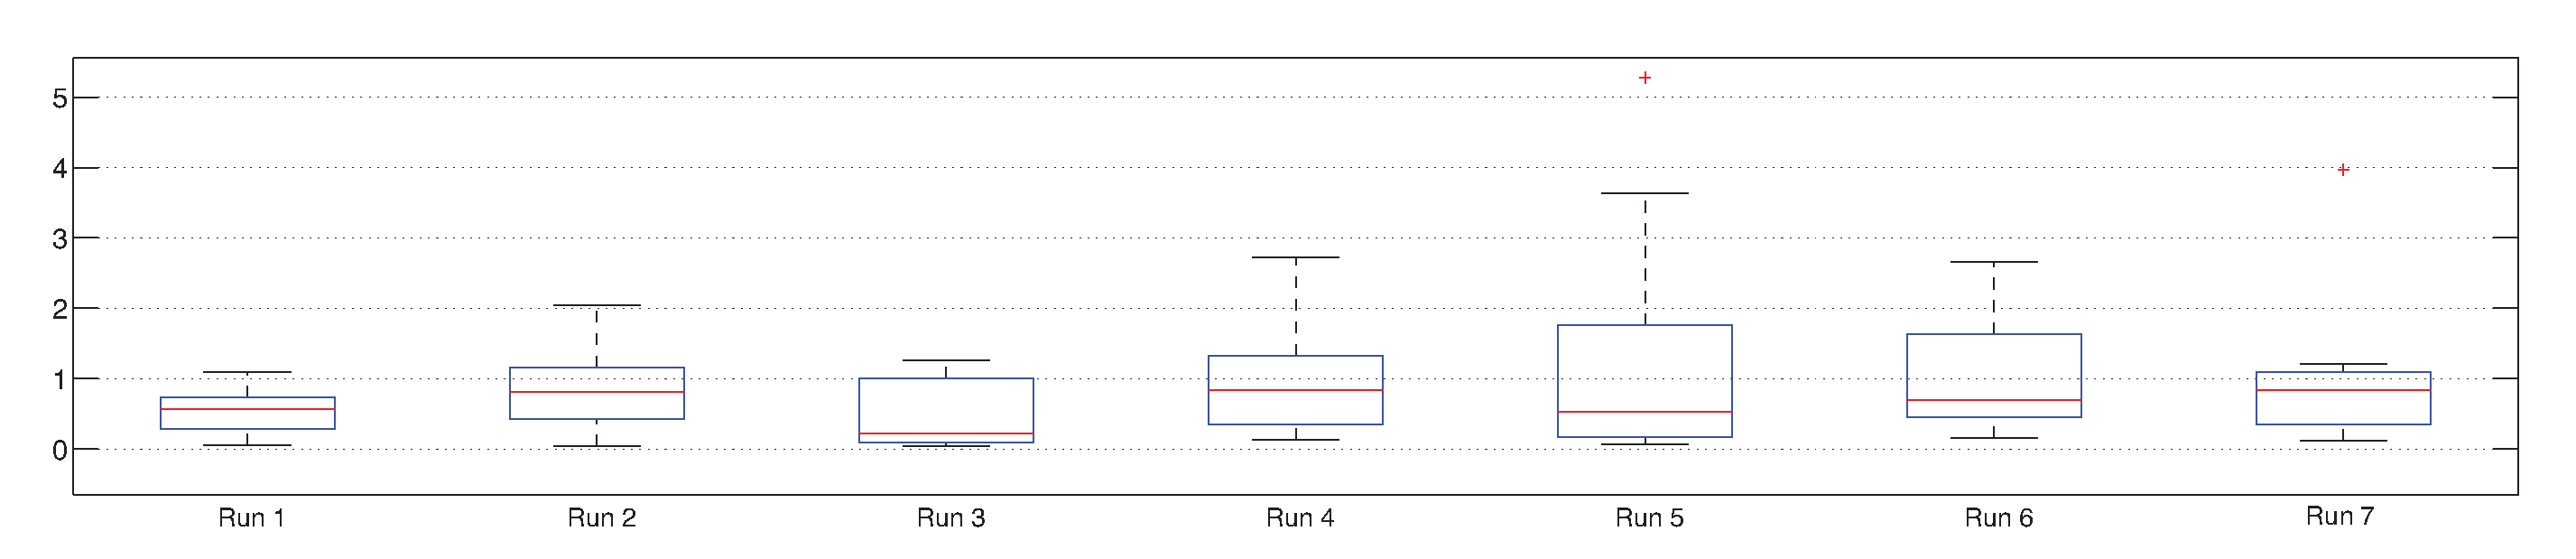
\includegraphics[width=1\textwidth]{./Figures/chapter6/data_collection/boxplot_results_real_world_runs.eps}
  \caption[Box plot results real-world runs individually optimized]{Box plot of the results for the real-world runs, indicating the number of data points between the actual and closest detected change points. A lower and more compact box plot is better.}
  \label{fig:boxplot_real_world_runs}
\end{figure}

This appendix provides observations and remarks which we made from inspecting the real-world results from \Cref{Chapter6}.
In \Cref{subsec:subjective_results} we have discussed a few overall effects.
In the following we discuss the performance of each run, using the (manually determined) specific parameters as listed in \Cref{tab:results_real_world}.

To give a better impression on the quality of the $d_{avg}$, \Cref{fig:boxplot_real_world_runs} shows a box plot for each run.
It shows the spread of the $d_{avg}$ in seconds over all the change points.
A lower and more compact box plot is better.

When looking at the individual runs, we have the following observations for each run:

\begin{enumerate}
  \item \textbf{Subject 2, straight walk and run} \Cref{fig:data_with_cps_run_1}
    \begin{itemize}
      \item The first transition from running to walking, around $14s$ is harder to discover than the transition for the same activities around $33s$.
      This shows is that in real-world applications there is a diversity between the same transitions and activities.
      \item Around $8s$, $9s$, and $16s$ a few steps (while walking) are regarded as change points.
      During the running segments from $17s$ and $28s$ there is a lower probability of change for each step.
    \end{itemize}
  \item \textbf{Subject 1, straight walk and run} \Cref{fig:data_with_cps_run_2}
    \begin{itemize}
      \item Following the video recordings, we have annotated a change point from running to walking around $37s$.
      Our method discovers a change point almost a second before.
      In retrospect, we can see that the data distribution indeed changes from the discovered change point on.
      This shows us two important principles.
      The first is that the annotations are subjective.
      The second is that between different activities the transition period is longer than we would think.
      Looking at the data, we can see that the body slows down, even before we visually notice it on the video recordings.
    \end{itemize}

  \item \textbf{Subject 2, walk and run around fountain} \Cref{fig:data_with_cps_run_3}
    \begin{itemize}
      \item Like in the first run, the walking segment from $24s$ results in a change point for each step.
      Further inspection of the data reveals that each step is indeed different from the other.
      Due to the global parameter settings, the sensitivity is too high for this segment to recognize it as one.
      It could also be that our used window-length is too small, to model a good representation of this segment.
      \item During the circular run, from $12s$ till $24$, there are two change points discovered.
      The difference for the rotational vectors need to accumulate to a certain value before they have enough influence to let the rotation be regarded as a change point.
    \end{itemize}
  \item \textbf{Subject 1, walk and run around fountain} \Cref{fig:data_with_cps_run_4}
    \begin{itemize}
      \item As with the other runs, the accelerometer data makes it harder to detect turns.
      It requires a higher sensitivity, which results in a higher \gls{far}.
    \end{itemize}
  \item \textbf{Subject 2, walk and run fountain 2} \Cref{fig:data_with_cps_run_5}
    \begin{itemize}
      \item During the standing segment around $38s$ there are a lot of false positives.
      It seems to be the \emph{false heterogeneity} problem described above.
    \end{itemize}
  \item \textbf{Subject 3, indoor stairs} \Cref{fig:data_with_cps_run_6}
    \begin{itemize}
      \item The walking segment around $22s$, between two segments of walking downstairs, shows little difference in the data.
      To recognize it as a change point a high sensitivity and low proximity time period $\delta$ is required.
      \item During some segments (downstairs from $24s$, upstairs from $42s$ and $54s$) the method discovers more change points than our annotation.
      A closer inspecting of the raw data reveals indeed changes in behavior.
      To exclude these (semi) false positives, a better tuning of parameters is required.
      \item Because of the circular shape of the stairs, the magnetic field sensors constantly differs.
      Although our method is build to exclude slow shifting changes (because we are only interested in sudden changes), with our used window width it still eventually results in change points.
      \item The difference between taking the stairs and walking is smaller than, \eg, walking and running.
      The delay between these segments seems to be larger, as illustrated around $33s$.
    \end{itemize}
  \item \textbf{Subject 2, walk around corner} \Cref{fig:data_with_cps_run_7}
    \begin{itemize}
      \item The $90^{\circ}$ counter-clockwise turn during the walking activity is hard to discover when the accelerometer sensor data is included.
      When only the magnetic field and rotation sensors are used, the turn requires a lower sensitivity.
      With only these two sensors all the other change points in this run are also successfully discovered.
    \end{itemize}
\end{enumerate}

\begin{figure}
  \centering
  \begin{subfigure}{1\textwidth}
    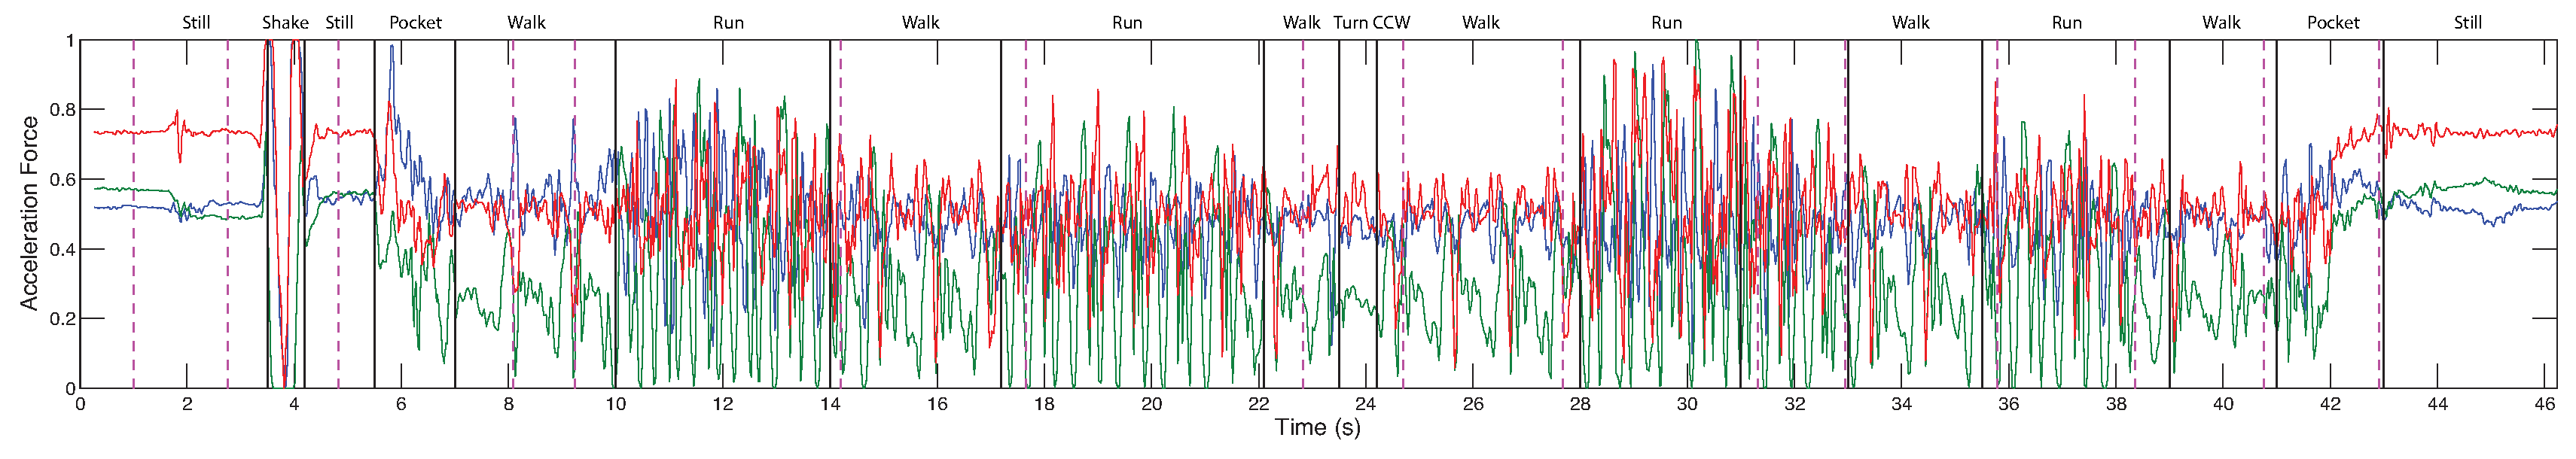
\includegraphics[width=\textwidth]{./Figures/chapter6/data_collection/run-1-walk-run-roemer/data_plot_acc_with_discovered_cps.eps}
    \caption{Run 1}
    \label{fig:data_with_cps_run_1}
  \end{subfigure}

  \begin{subfigure}{1\textwidth}
    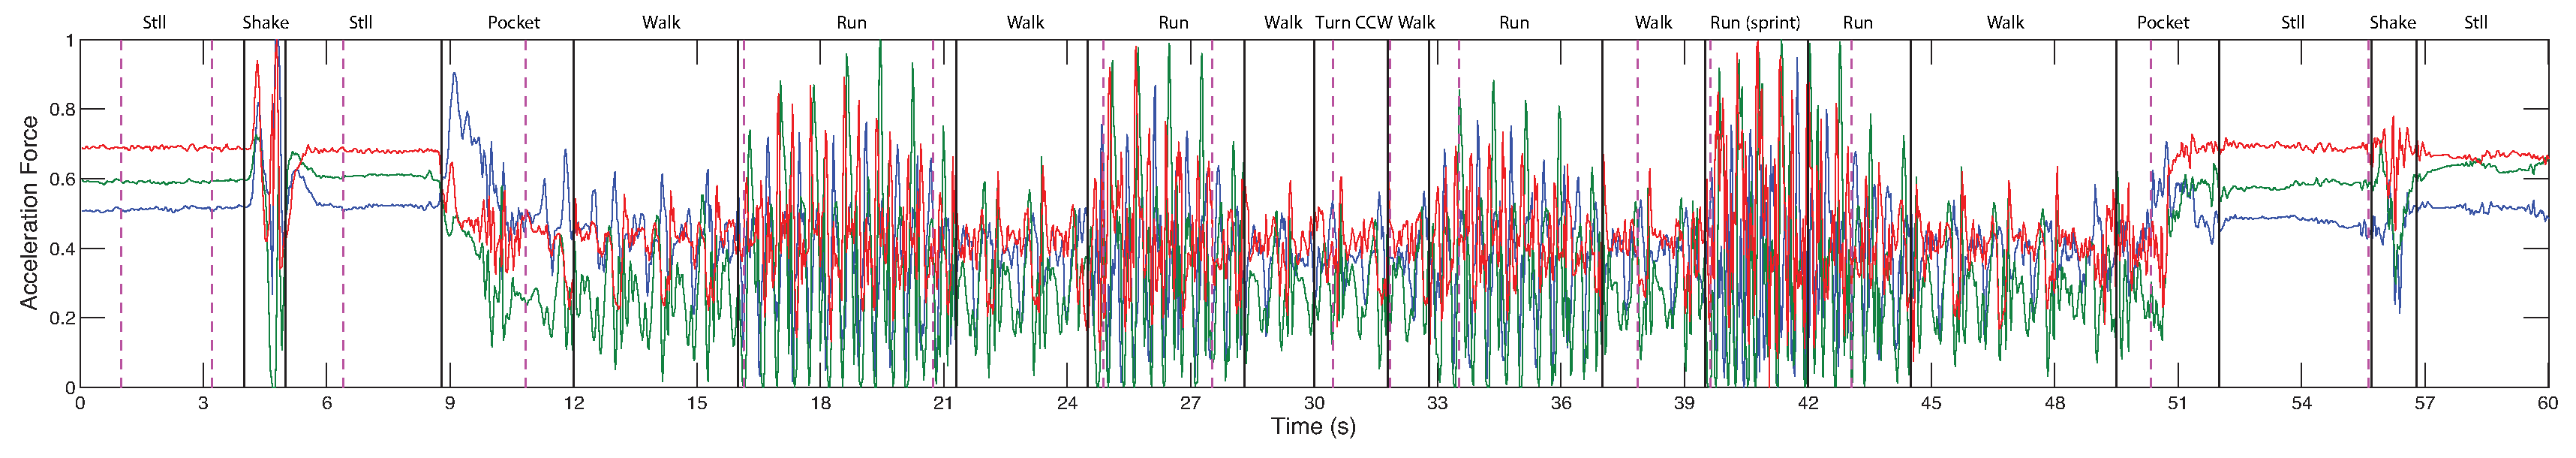
\includegraphics[width=\textwidth]{./Figures/chapter6/data_collection/run-2-walk-run-jos/data_plot_acc_with_discovered_cps.eps}
    \caption{Run 2}
    \label{fig:data_with_cps_run_2}
  \end{subfigure}

  \begin{subfigure}{1\textwidth}
    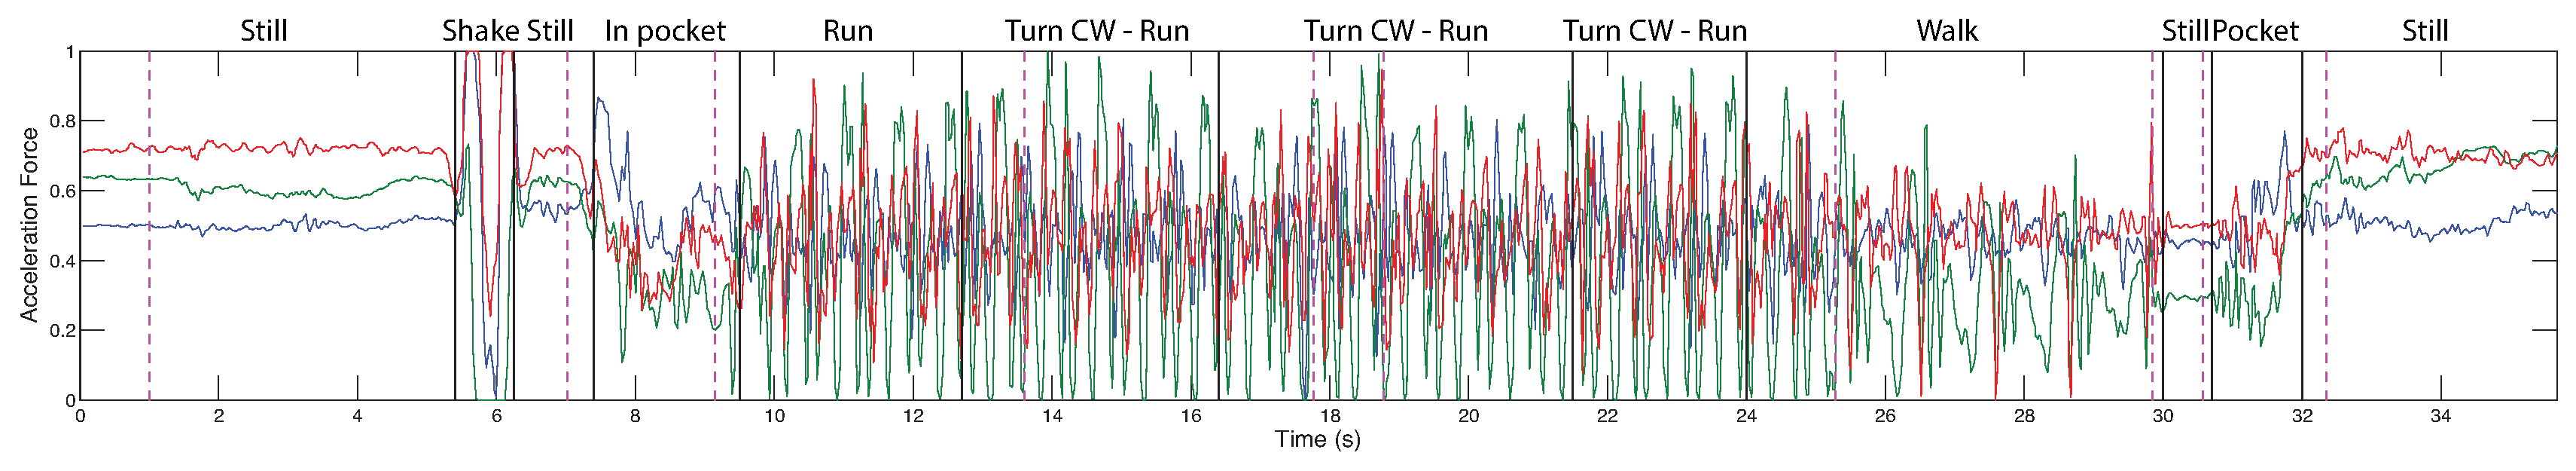
\includegraphics[width=\textwidth]{./Figures/chapter6/data_collection/run-4-run-fountain-roemer/data_plot_acc_with_discovered_cps.eps}
    \caption{Run 3}
    \label{fig:data_with_cps_run_3}
  \end{subfigure}

  \begin{subfigure}{1\textwidth}
    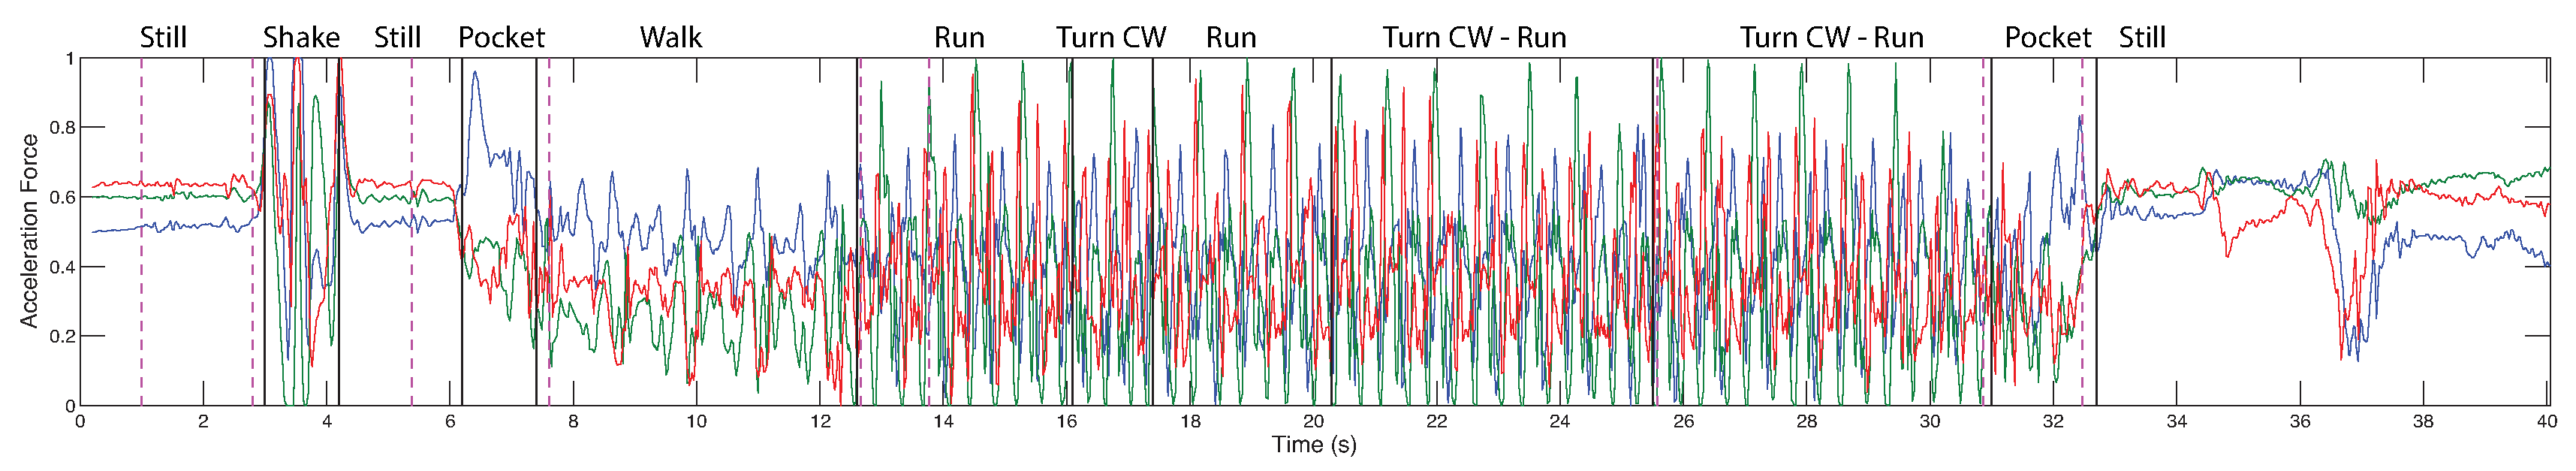
\includegraphics[width=\textwidth]{./Figures/chapter6/data_collection/run-5-run-fountain-jos/data_plot_acc_with_discovered_cps.eps}
    \caption{Run 4}
    \label{fig:data_with_cps_run_4}
  \end{subfigure}

  \begin{subfigure}{1\textwidth}
    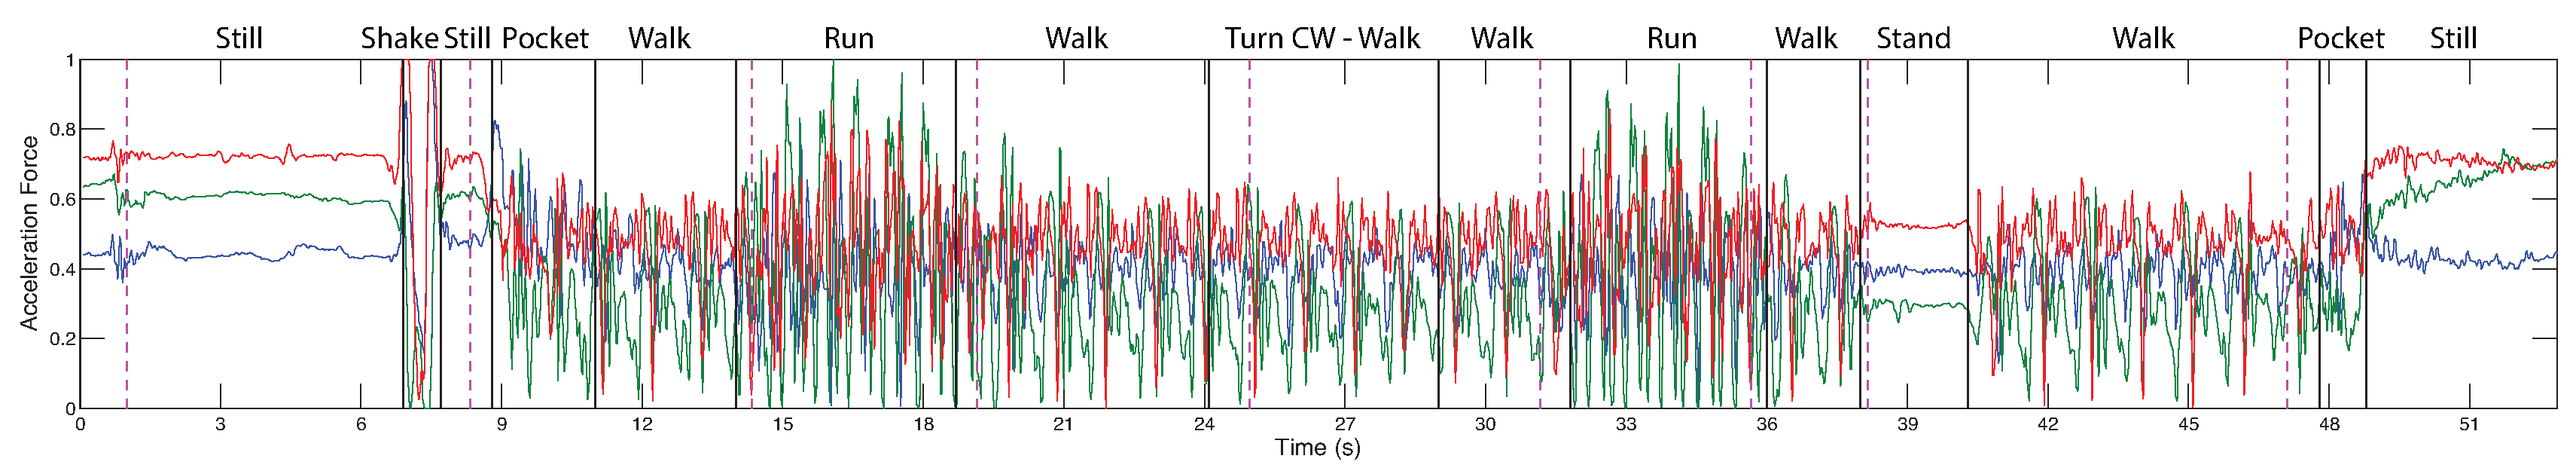
\includegraphics[width=\textwidth]{./Figures/chapter6/data_collection/run-6-walk-run-roemer/data_plot_acc_with_discovered_cps.eps}
    \caption{Run 5}
    \label{fig:data_with_cps_run_5}
  \end{subfigure}

  \begin{subfigure}{1\textwidth}
    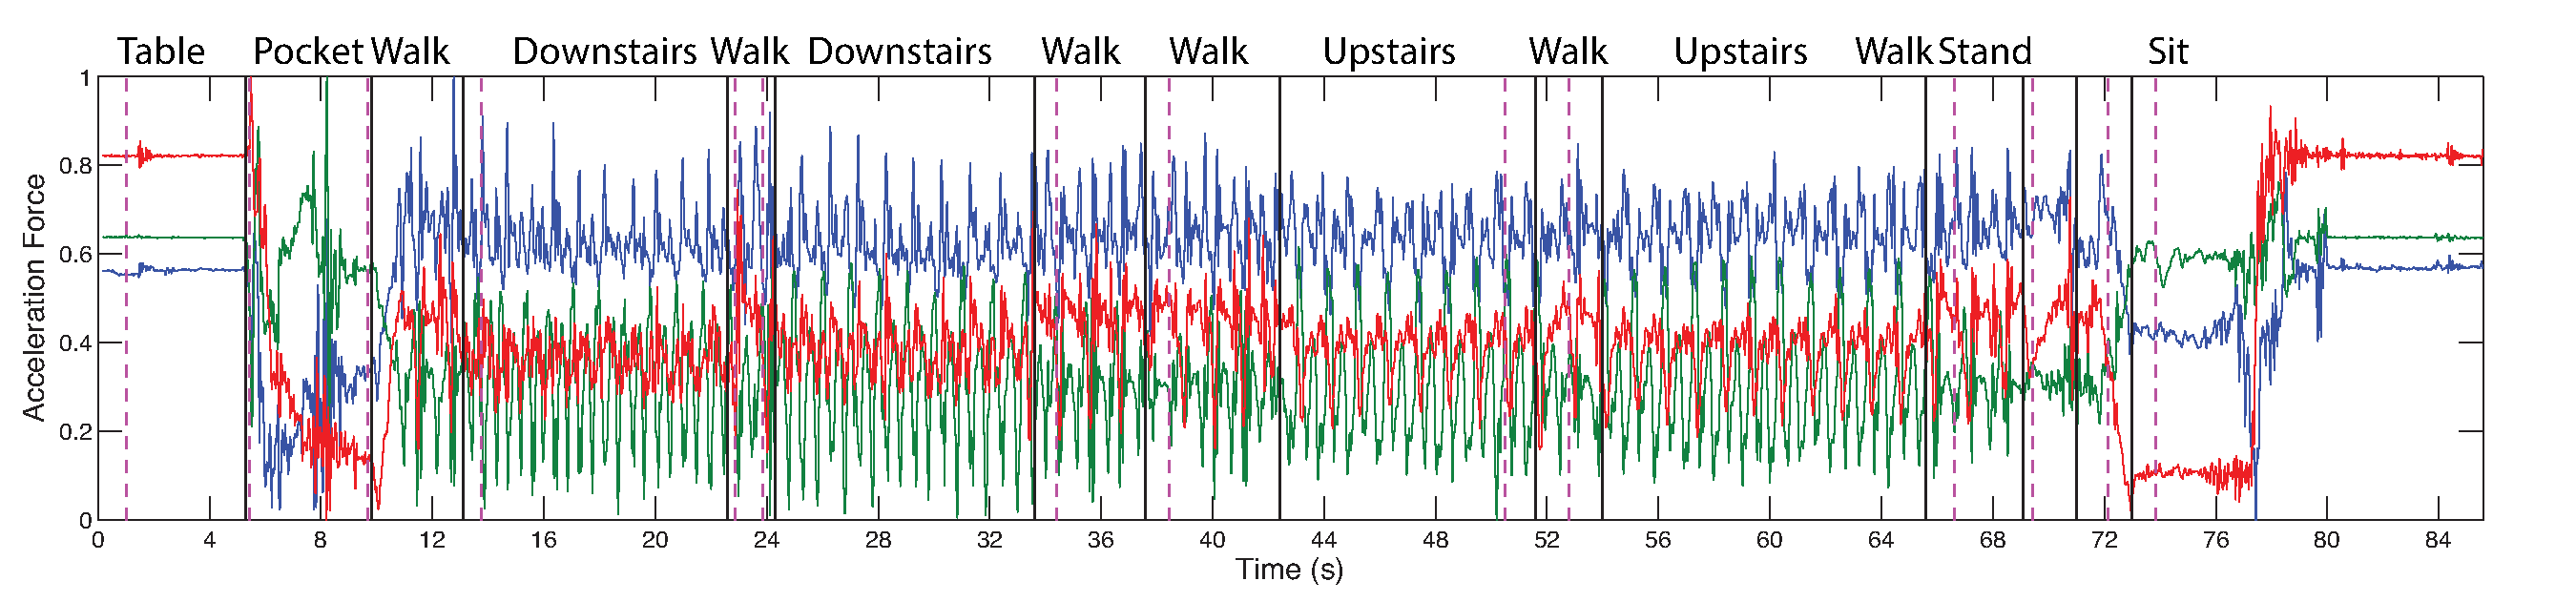
\includegraphics[width=\textwidth]{./Figures/chapter6/data_collection/stairs-1-marc/data_plot_acc_with_discovered_cps.eps}
    \caption{Run 6}
    \label{fig:data_with_cps_run_6}
  \end{subfigure}

  \begin{subfigure}{1\textwidth}
    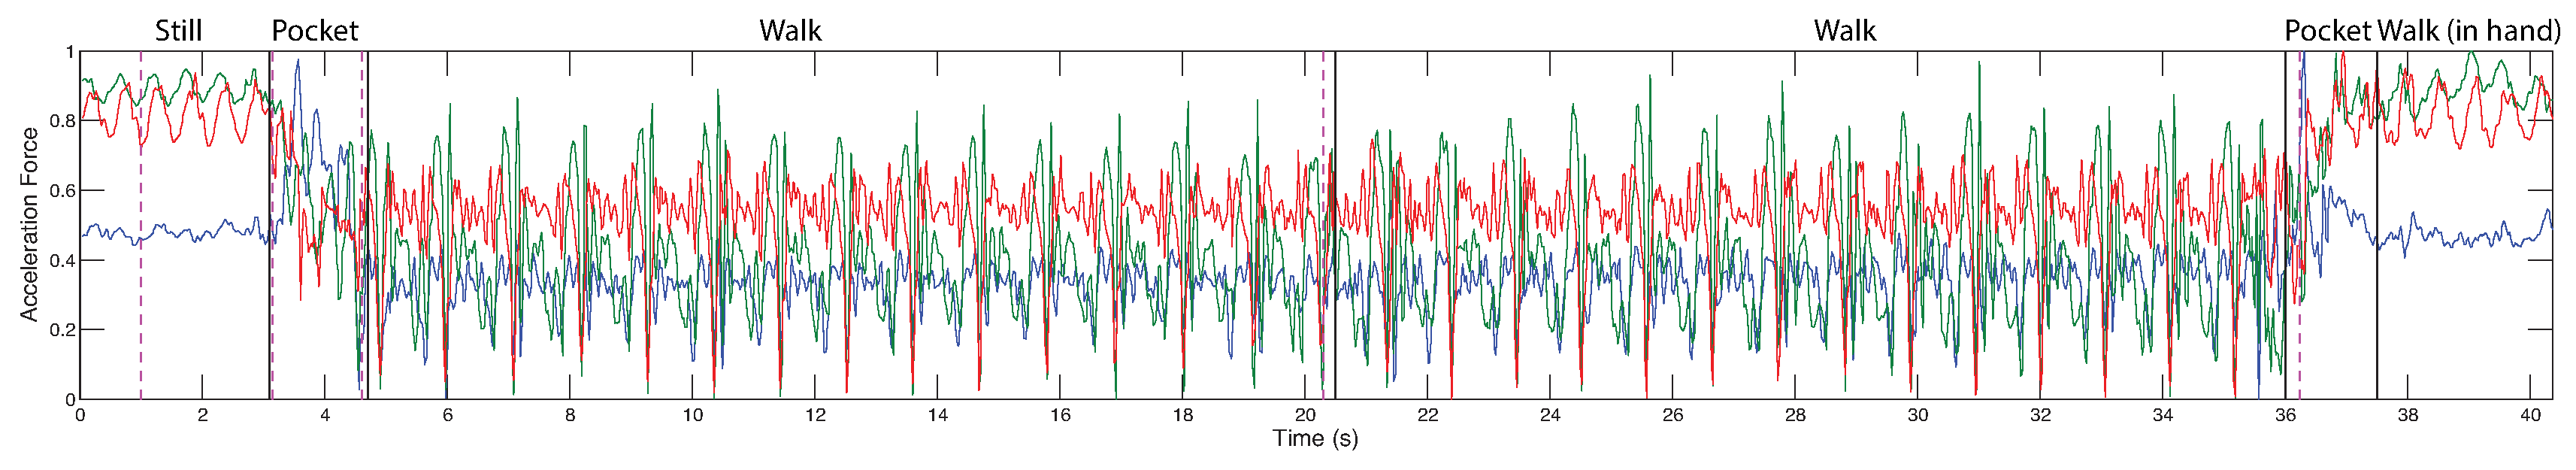
\includegraphics[width=\textwidth]{./Figures/chapter6/data_collection/run-3-walk-turn-roemer/data_plot_acc_with_discovered_cps.eps}
    \caption{Run 7}
    \label{fig:data_with_cps_run_7}
  \end{subfigure}

  \caption[Results run 1/8]{Annotated plots of all runs. The black vertical lines are manually determined change points, the purple dashes lines are the discovered change points. The label above each segment indicates the current performed activity.}\label{fig:plots_all_runs_results}
\end{figure}